% 1977 年北京卷文科第 10 题：二次函数图象
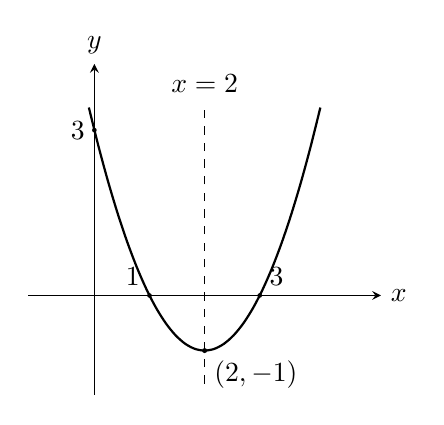
\begin{tikzpicture}[scale=0.7,>=stealth]
  \draw[->] (-1.2,0)--(5.2,0) node[right] {$x$};
  \draw[->] (0,-1.8)--(0,4.2) node[above] {$y$};
  \draw[thick,domain=-0.1:4.1,smooth,variable=\x]
    plot ({\x},{(\x-2)^2-1});
  \fill (2,-1) circle (1.3pt) node[below right] {$\left(2,-1\right)$};
  \fill (1,0) circle (1.2pt) node[above left] {$1$};
  \fill (3,0) circle (1.2pt) node[above right] {$3$};
  \fill (0,3) circle (1.2pt) node[left] {$3$};
  \draw[dashed] (2,-1.6)--(2,3.5) node[above] {$x=2$};
\end{tikzpicture}
